\documentclass[a4paper,12pt]{scrartcl}
\usepackage{xcolor}
\usepackage[UKenglish]{isodate}%http://ctan.org/pkg/isodate
\usepackage[a4paper,left=2cm, right=2cm,top=2.7cm, bottom=3cm]{geometry}
\usepackage{changepage}
\usepackage{fancyhdr}
\usepackage[export]{adjustbox}
\usepackage{sectsty}
\usepackage[titles]{tocloft}
\usepackage{hyperref}
\usepackage{graphicx}
\hypersetup{
    colorlinks,
    citecolor=black,
    filecolor=black,
    linkcolor=black,
    urlcolor=black
}

\hyphenchar\font=-1
\setlength{\cftbeforesecskip}{4pt}

\newenvironment{subs}
{\adjustwidth{3em}{0pt}}
{\endadjustwidth}
\renewcommand{\cftsecleader}{\cftdotfill{\cftdotsep}}
\renewcommand{\familydefault}{\sfdefault}

\pagestyle{fancy}
\fancyhf{}
\renewcommand{\headrulewidth}{0pt}
\lhead{\today}
\chead{System Design Document}
\rhead{\ProjectName}
\lfoot{
\includegraphics[scale=0.147,valign=c]{EIST.png}}
\cfoot{\thepage}
\rfoot{
\includegraphics[scale=0.4,valign=c]{TUM.png}}

\newcommand{\ProjectName}{TUM Social}

\begin{document}
    \section*{Purpose}
    The system design is documented in the System Design Document (SDD). It describes additional design goals set by the software architect, the subsystem decomposition (with UML class diagrams), hardware/software mapping (with UML deployment diagrams), data management, access control, control flow mechanisms, and boundary conditions. The SDD serves as the binding reference document when architecture-level decisions need to be revisited.

    \section*{Audience}
    The audience for the SDD includes the system architect and the object designers as well as the project manager.
    \nopagebreak

    \renewcommand{\contentsname}{Table of Contents}
    \tableofcontents
    \section*{Document History}

    \begin{tabular}{
        |p{\dimexpr.08\linewidth-2\tabcolsep-1.3333\arrayrulewidth}% column 1
        |p{\dimexpr.17\linewidth-2\tabcolsep-1.3333\arrayrulewidth}% column 2
        |p{\dimexpr.20\linewidth-2\tabcolsep-1.3333\arrayrulewidth}
        |p{\dimexpr.56\linewidth-2\tabcolsep-1.3333\arrayrulewidth}|% column 3
    }
        \hline
        Rev. & Author & Date            & Changes          \\
        \hline
        1    & Luis Traffa  & 9th July 2022 & Everything \\
       
        \hline
    \end{tabular}
    \newpage
    \sectionfont{\color[HTML]{355a8a}}  % sets colour of chapters
    \subsectionfont{\color[HTML]{4e81bc}}


    \section{Introduction}
    
    \subsection{Overview}
        
    The system is essentially a standard client server application. The client is a webbrowser like Firefox or Chrome, which connects to the TUM SOCIAL server and makes requests from it.
    The server handles these rquests and sends the responses back to the server. 

     


    \section{Design Goals}
    
    When designing the system we had certain non-functional requirements in mind. We determined the most important of these to be scalability, usability and maintainablility. These fundamental priciples shaped the development of our system and are easily noticed by users. Our registration process is very simple and new users can sign up with just a couple clicks and have full access to all the features right away. Furthermore, the database is highly capable and enables the network to expand and support a growing number of users. The code is also easy to read as the system uses the MVC pattern with various different controllers for different features.


    \section{Subsystem Decomposition}
    This section describes the decomposition of the system into subsystems and the services provided by each subsystem. The services are the seed for the APIs detailed in the Object Design Document. The system can generally be seperated into 3 distinct components. The database, server and client. The database stores all data and offers a facade interface to let the server request data. The server is a standard spring boot application, which handles all of the clients requests. The client provides the end user with a GUI, that makes use of various controllers for different functions, to make requests from the server. The following diagram is a rough representation of the system seperated into its basic components/subsystems.\\
    	
    	
        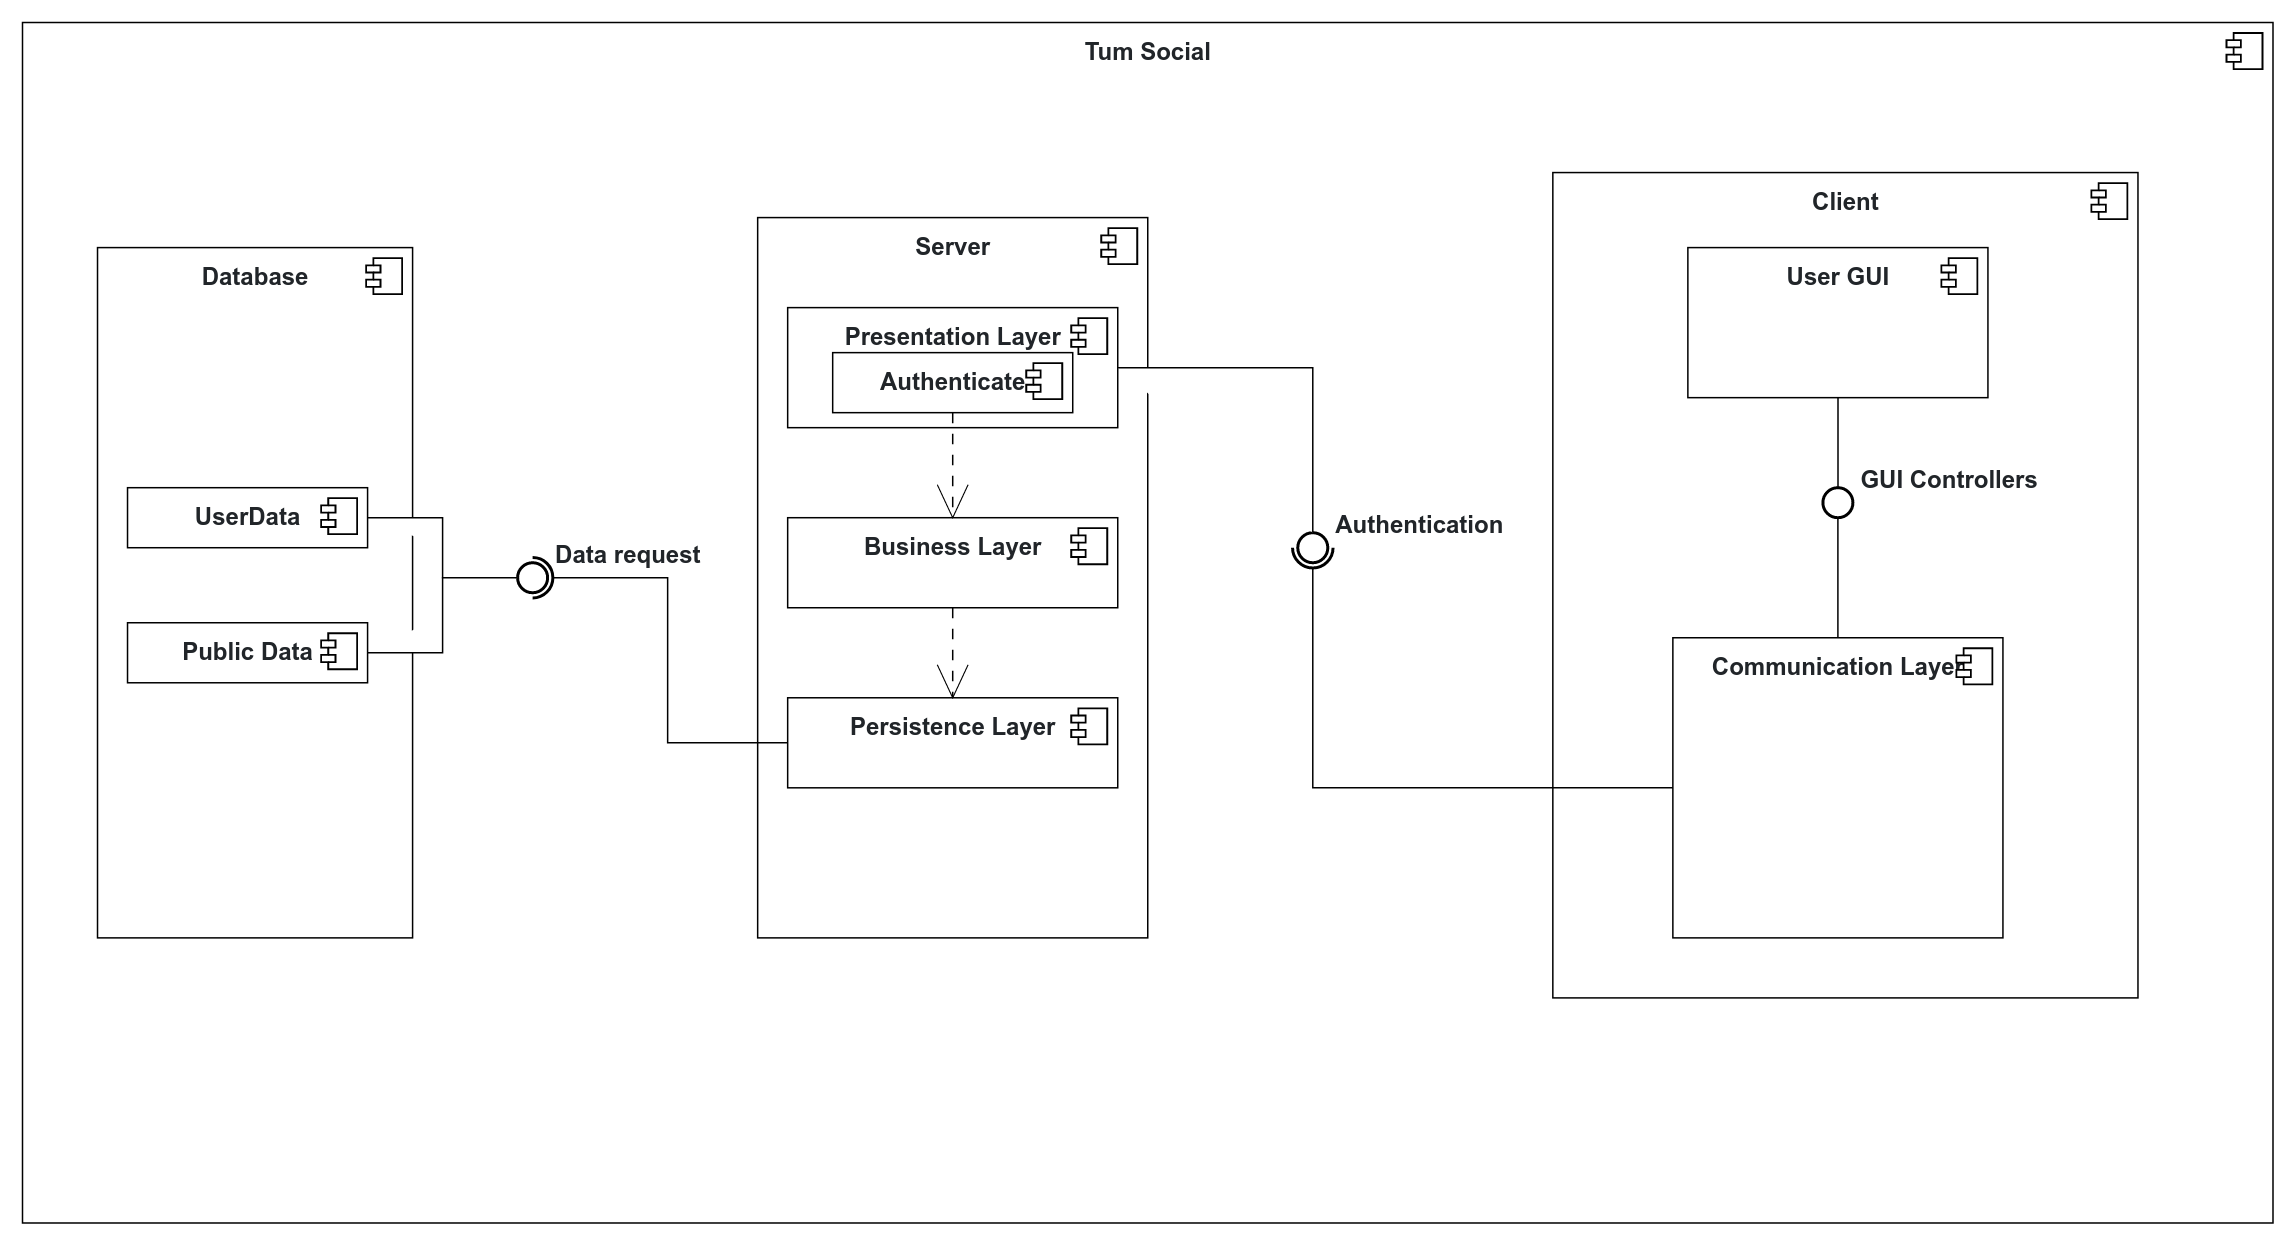
\includegraphics[scale=0.15]{ComponentDiagram.png}
  


    \section{Hardware/Software Mapping}
In physical space the subsystems are distrubuted on 2 seperate hardware nodes. The client machine and the server machine. The client machine only contains the view, which is displays the current state of the model and is updated by controllers when the user sends requests to the server. There exist several different kinds of controllers. One for each core aspect of the system like the profile or chat. The controllers provide services that the models need to get the data and display it. The database is also located on the server node. The protocol employed is the standard https, which comes with Spring boot.\\
    
    
    
    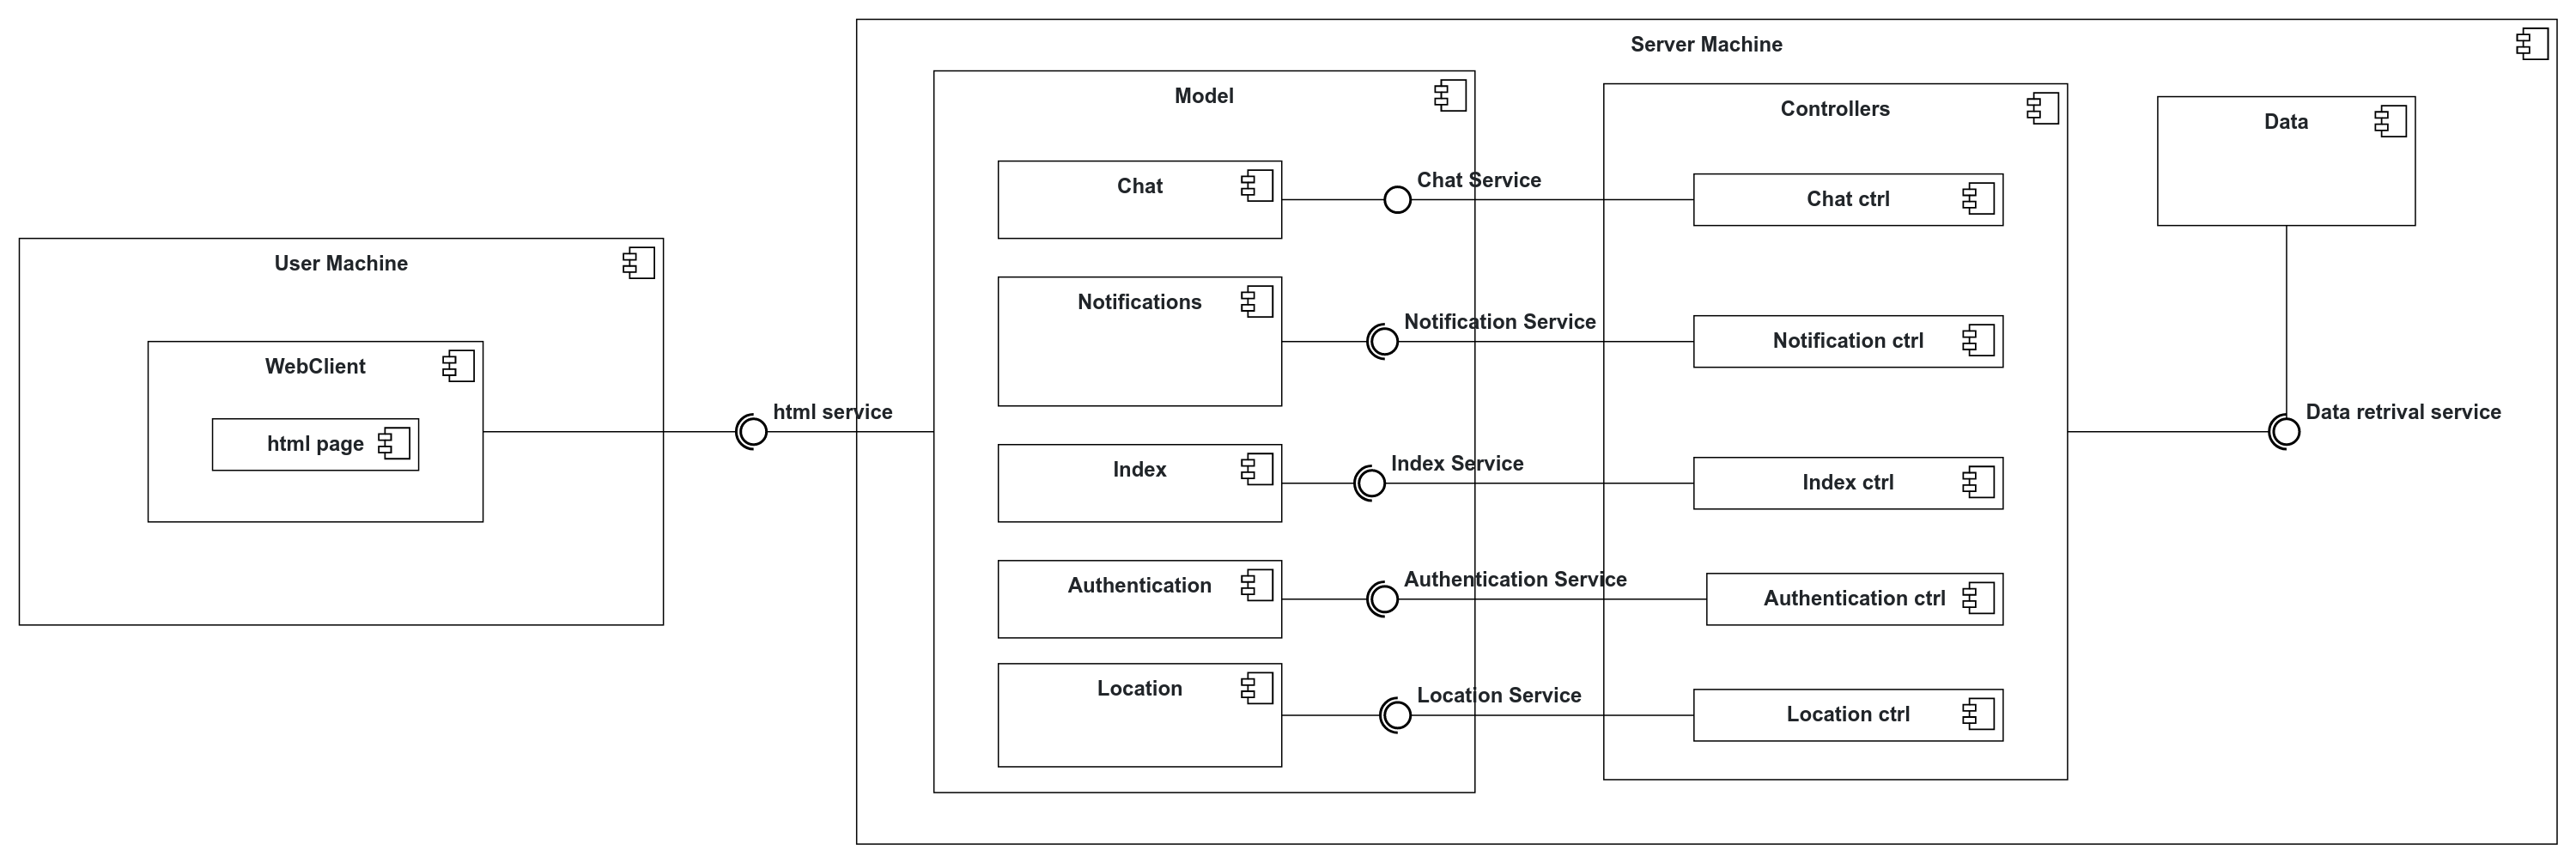
\includegraphics[scale=0.15]{HardwareSoftware.png}
    
    


    \section{Persistent Data Management}
    This section describes how the entity objects are mapped to persistent storage.
    It contains a rationale of the selected storage scheme, file system or database, a description of the selected database and database administration issues.


    \section{Access Control and Security}
    This section describes the access control and security issues based on the nonfunctional requirements in the requirements analysis document. It also describes the implementation of the access matrix based on capabilities or access control lists, the selection of authentication mechanisms and the use of encryption algorithms.\\
    
    All sensitive user data, namely the password, is stored in the database only in a hashed state. Therefore 


    \section{Global Software Control}
    
    The design of TUM Social is highly centralized. All data is stored on the server and if someone were to seize control of the server, that person would have full control over the network.
    Furthermore, the system is a polling based design, which means that the server is continuously polling for new requests and doesnt shut-off when it does not need to do anything, like an event-			based system would. Requests are initaited when an end-user makes a request through a running client. 


    \section{Boundary Conditions}
   First of all the server needs to be started, as it handles all of the communication within the network. When the server is running clients can start up and try to connect to it. If a connection cannot be successfully made, clients will simply have to retry until the server responds. Ideally the server is running continously, but it is possible that at somepoint the server stops answering requests. This may be because of a "distributed denial-of-service" attack or technical problems. When this happens the clients will not be able to communicate with each other. All connected clients will experience a lack of response from the server. The clients will have to wait until the server is operational again. If at some point the system is supposed to shut sown indefinitly, the clients should end the connection with the server before it will shutdown.\\

\end{document}
